\chapter{Introduction}\label{chap:Intro}


The proton is one of the basic building blocks of ordinary matter and, at the same time, a highly complex system. It is a composite particle made of quarks and gluons, with a valence-quark content of two up quarks and one down quark, bound together by the strong interaction. While its constituents and their interactions are described by quantum chromodynamics (QCD), many properties of the proton cannot be obtained straightforwardly from perturbative calculations. Precise measurements of its electromagnetic properties therefore provide valuable information about its structure and are essential for testing our theoretical understanding of the proton.

Since the electric charge of the proton is distributed over a finite volume rather than concentrated at a single point, its spatial extent can be characterized by the proton charge radius. The electromagnetic structure of the proton is described by form factors, which parameterize its charge and magnetization distributions. In particular, the electric Sachs form factor \(G_E(Q^2)\) describes the electric structure of the proton as a function of the squared four-momentum transfer \(Q^2\). Its slope at zero momentum transfer is directly related to the proton charge radius,
\[
r_p^2 =
-6
\left.
\frac{dG_E(Q^2)}{dQ^2}
\right|_{Q^2=0}.
\]
A precise determination of the proton charge radius therefore requires measurements at very small momentum transfers and an accurate extrapolation of the electric form factor towards \(Q^2=0\).

Experimentally, the proton charge radius can be determined using two different approaches. The first is based on spectroscopy, in which atomic energy differences are determined by measuring the absorption or emission of electromagnetic radiation. A particularly sensitive observable is the Lamb shift. In the Dirac description of hydrogen with a point-like proton, the \(2S_{1/2}\) and \(2P_{1/2}\) states are degenerate. However, in 1947, Lamb and Retherford experimentally demonstrated that the \(2S_{1/2}\) state lies slightly above the \(2P_{1/2}\) state in energy. This observation played an important role in the development of quantum electrodynamics (QED), which explains most of this energy difference through radiative corrections.

The proton charge radius introduces an additional contribution to these atomic energy levels. This effect is especially important for \(S\)-states, whose wave functions have a non-zero probability density at the position of the proton and therefore overlap with its charge distribution. The \(2P\)-state, in contrast, has a vanishing probability density at the origin and is affected much less. As a result, the measured energy difference between the \(2S\) and \(2P\) states also contains information about the proton charge radius. By comparing precisely measured transition frequencies with theoretical predictions, the proton radius can therefore be extracted.

Measurements of the Lamb shift in muonic hydrogen provide an especially precise determination of the proton radius. Muonic hydrogen is a hydrogen-like atom in which the electron is replaced by a negatively charged muon. Due to the much larger mass of the muon compared to the electron, its Bohr radius is approximately 200 times smaller than that of ordinary hydrogen. As a result, the muon has a significantly larger probability density close to the proton, making the energy levels much more sensitive to the finite proton size.

The second approach uses elastic lepton--proton scattering experiments, where the differential scattering cross section provides access to the proton's electromagnetic form factors. More details on this approach will be discussed in Chapter~\ref{chap:Theory}.

Historically, measurements based on elastic electron--proton scattering and spectroscopy of ordinary hydrogen yielded a proton charge radius of approximately \(0.88\,\mathrm{fm}\). This picture changed significantly in 2010, when a high-precision measurement of the Lamb shift in muonic hydrogen led to a significantly smaller value of approximately \(0.84\,\mathrm{fm}\). The discrepancy between this result and previous determinations became known as the proton radius puzzle. Figure \ref{fig:PCR} illustrates this discrepancy and summarizes several experimental determinations of the proton charge radius.

\begin{figure}[h]
    \centering
    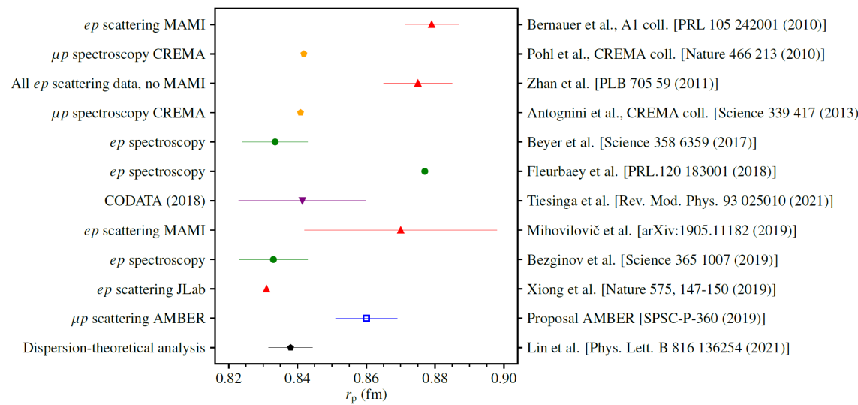
\includegraphics[width=0.9\textwidth]{figures/PCR.pdf}
    \caption{Comparison of proton charge radius measurements from different experiments. Figure taken from \cite{Karl PAW25}.}
    \label{fig:PCR}
\end{figure}

Although more recent measurements have substantially reduced the discrepancy, an independent high-precision determination of the proton radius remains important. In this context, elastic muon--proton scattering provides such an independent approach. A new precision measurement using this method is pursued by the AMBER experiment at CERN, which will be presented in detail in \autoref{chap:AMBER}.